\documentclass[11pt,a4paper]{ltjsarticle}
\usepackage[haranoaji]{luatexja-preset}
\usepackage{amsmath,amssymb}
\usepackage{graphicx}
\usepackage{booktabs}
\usepackage{array}
\usepackage[margin=25mm]{geometry}
\usepackage{siunitx}
\usepackage{caption}
\usepackage{authblk}
\usepackage[hidelinks]{hyperref}
\usepackage{xcolor}

\graphicspath{{../}}
\captionsetup{font=small,labelfont=bf}
\allowdisplaybreaks

% ショートハンド
\newcommand{\bra}[1]{\langle #1|}
\newcommand{\ket}[1]{|#1\rangle}
\newcommand{\ev}[1]{\langle #1\rangle}
\newcommand{\Tr}{\operatorname{Tr}}
\newcommand{\Var}{\operatorname{Var}}
\newcommand{\Cov}{\operatorname{Cov}}
\newcommand{\Pf}{\operatorname{Pf}}
\newcommand{\gd}{\gamma}

\title{\bfseries 共通ランダム測定 (CRM) によるハバード模型の\\測定効率化: 平均場priorから matchgate シャドウまで}
\author{龍山 昊平}
\affil{\normalsize（本稿は数値実験ノートを論文形式にまとめた作業原稿。著者名・所属は適宜編集のこと。）}
\date{2026年7月19日}

\begin{document}
\maketitle

\begin{abstract}
古典シャドウ(ランダム測定)に古典計算で得た近似状態(prior)を組み合わせて測定分散を削減する共通ランダム測定 (common randomized measurements, CRM)[Vermersch \textit{et al.}, PRX Quantum \textbf{5}, 010352 (2024)] を、フェルミオン・ハバード模型へ系統的に適用した。局所 Pauli 観測量に対する CRM の分散削減率(利得 $G$)が、prior のグローバル忠実度ではなく\emph{観測量ごとの局所誤差} $\Delta$ のみで決まる閉形式で与えられることを示し、これを約 5 桁($G\approx 5\times10^{-3}$--$10^{3}$)にわたり数値検証した。帰結として、prior のグローバル忠実度が系サイズとともに指数的に崩壊する領域($L=32$ 鎖で $F=0.007$)でも局所観測量の利得は保たれることを 64 量子ビット規模で実証した。さらに、Wick の定理により \emph{MPS 表現を要さない} $O(N^3)$ の非制限 Hartree--Fock (UHF) 平均場 prior を導入し、2 次元シリンダー(最大 96 量子ビット、研究室クラスターでの DMRG 計算)においてこれが $\chi=32$--$64$ の切断 MPS prior に匹敵すること、その弱点(サイト間スピン相関)がスピン回転平均した\emph{混合状態} prior で修復されることを示した。CRM を制御変量法の一般形へ拡張し、係数をデータから推定することで「priorがどれほど悪くても損をしない」($G\ge 1$)推定器を構成した。また matchgate(フェルミオン Gauss)シャドウにより Jordan--Wigner 弦の問題を解消し 2 次元の全エネルギー測定を可能にする一方、CRM の利得は測定アンサンブルに依存し自己平均的な Gauss 測定にはほとんど効かないことを定量化した。最後に、これらを統合して「安価な prior の相図」— 平均場 prior が有効な物理領域と、広幅ドープ系の電荷テクスチャで破綻する境界 — を確定した。
\end{abstract}

\tableofcontents

\section{序論と問い}

量子シミュレータや量子コンピュータで用意した状態 $\rho$ から物理量 $\ev{O}$ を精度 $\epsilon$ で推定するには、一般に $O(1/\epsilon^2)$ 回の測定が必要であり、これが多くの応用でコストの支配項となる。古典シャドウ(ランダム測定)[Huang, Kueng, Preskill, Nat.\ Phys.\ \textbf{16}, 1050 (2020)] は、ランダムに選んだ測定基底の記録から多数の物理量を後処理で同時推定できる強力な枠組みだが、ランダム化ゆえに個々の物理量に対する分散は素朴な直接測定より大きい。

共通ランダム測定 (CRM) は、実験状態 $\rho$ の古典的近似 $\sigma$(prior)を用意し、\emph{同一}のランダムユニタリ $u$ を $\sigma$ にも古典計算で適用して差分を取ることで、ランダム化に由来する分散を打ち消す:
\begin{equation}
  \hat o_{\rm CRM} = \frac{1}{n_u}\sum_u \bigl[\,\overline{X_\rho(u)} - X_\sigma(u)\,\bigr] + \Tr[O\sigma].
  \label{eq:crm}
\end{equation}
差分を取っても期待値は不変だが、同一の $u$ を用いるため「ランダム基底の選び方」に由来する揺らぎが $\rho$ 側と $\sigma$ 側で相関し、差で相殺される。原論文は汎用の行列積状態 (MPS) prior を扱うが、フェルミオン系への応用では次の問いが残っていた。
\begin{itemize}
  \item \textbf{Q1:} Hartree--Fock などの標準的な近似は prior としてどこまで有効か。大きい系では近似精度(グローバル忠実度)が指数的に落ちるが、それでも手法に意味はあるか。
  \item \textbf{Q2:} MPS が高くつく 2 次元系で、安価な平均場 prior は $\chi$ 制限 MPS prior に代われるか。
\end{itemize}
本稿の結論を先取りすると、\textbf{利得はグローバル忠実度ではなく観測量ごとの局所誤差 $\Delta$ で決まる}(第\ref{sec:gainlaw}節)。したがって Q1 は「局所観測量に対しては有効」、Q2 は「オンサイト量では代われ、対称性回復すればほぼ全観測量で代われる」と答えられる(第\ref{sec:2d}節)。

\section{手法}
\label{sec:methods}

\subsection{模型と量子ビットへの写像}
ハバード模型
\begin{equation}
  H = -t\!\!\sum_{\langle ij\rangle\sigma}\!\!\bigl(c^\dagger_{i\sigma}c_{j\sigma}+\text{h.c.}\bigr) + U\sum_i n_{i\uparrow}n_{i\downarrow} - \mu\sum_{i\sigma}n_{i\sigma}
\end{equation}
を $t=1$、原則 half-filling($\mu=U/2$、粒子数は保存量として固定)で扱う。Jordan--Wigner (JW) 変換の順序はサイト $s$ の $\uparrow$ を量子ビット $2s-1$、$\downarrow$ を $2s$ とする。密度・スピン $z$ 型の観測量($n,\ nn,\ S^zS^z$)は JW 後も $Z$ 列のままで台のサイズ $|A|=1$--$2$ に留まる一方、ホッピング $c^\dagger_a c_b+\text{h.c.}$ は $(XZ\cdots ZX + YZ\cdots ZY)/2$ となり JW 順序上の距離だけ台が伸びる(1 次元最近接で $|A|=3$、2 次元の $x$ 方向ボンドで $|A|=2W+1$)。後者は第\ref{sec:matchgate}節の主題となる。

\subsection{CRM 推定器と prior 側の厳密化}
各「設定」$u$ で各量子ビットの測定基底を $X/Y/Z$ から独立一様に選び $n_m$ ショット測定する。これを $n_u$ 設定繰り返す(総ショット数 $n_u n_m$)。Pauli 列 $P$(台 $A$)のスナップショット推定値は「基底が $A$ 上で全一致したときのみ $3^{|A|}\times(\pm1)$、不一致なら厳密に $0$」となる。

先行実装では \eqref{eq:crm} の $\sigma$ 側も有限ショットでサンプルしており、その独立ノイズ $V_s^{(\sigma)}/n_m$ が上乗せされてショットノイズ支配域で CRM が標準シャドウに\emph{負けていた}。本研究の出発点はこれを厳密計算に修正することであった。局所 Pauli に対し prior 側の条件付き期待値は閉形式
\begin{equation}
  E[X_\sigma\,|\,u] = \sum_t c_t\,\mathbf{1}[\text{基底一致}]\,3^{|A_t|}\,\ev{P_t}_\sigma
  \label{eq:priorexact}
\end{equation}
で与えられ、必要なのは項ごとの $\ev{P_t}_\sigma$ のみである。この事実が「MPS でなくとも Wick の定理で書ける状態なら何でも prior になる」「混合状態でもよい」という後の展開の鍵となる。

\subsection{分散の閉形式と利得法則}
\label{sec:variance}
ランダム Pauli 測定では、基底が台 $A$ 上で一致する確率が $3^{-|A|}$、一致時のスナップショット値が $3^{|A|}\times(\pm1)$、不一致時は厳密に $0$ であることから、
\begin{align}
  V_u &= (3^{|A|}-1)\,\ev{P}^2 && (\text{ユニタリ揺らぎ}),\\
  E_u[\Var(X|u)] &= 3^{|A|}\bigl(1-\ev{P}^2\bigr) && (\text{条件付きショットノイズ}).
\end{align}
CRM は $\ev{P}^2$ を $\Delta^2$ に置き換え、ショットノイズは不変に残す。ここで
\begin{equation}
  \Delta \equiv \ev{P}_\rho - \ev{P}_\sigma
\end{equation}
は prior の\emph{局所}誤差である。したがって利得
\begin{equation}
  \boxed{\;G = \frac{(3^{|A|}-1)\,\ev{P}^2 + v_s}{(3^{|A|}-1)\,\Delta^2 + v_s},\qquad v_s = \frac{3^{|A|}\bigl(1-\ev{P}^2\bigr)}{n_m}\;}
  \label{eq:gainlaw}
\end{equation}
が得られる。\eqref{eq:gainlaw} には prior のグローバル忠実度が\emph{一切現れない}。$\Delta\to0$ の上限として飽和則
\begin{equation}
  G_{\max}(n_m) = 1 + n_m\,\frac{(3^{|A|}-1)\ev{P}^2}{3^{|A|}(1-\ev{P}^2)}
  \label{eq:saturation}
\end{equation}
が従い、CRM は「少ない設定 $\times$ 多ショット」の予算配分で最大化される。なお多項観測量(例: 二重占有 $=\tfrac14(I-Z_\uparrow-Z_\downarrow+Z_\uparrow Z_\downarrow)$)の利得は合計 $\Delta$ だけでなく\emph{項ごとの} $\Delta$ に依存する。参照状態が対称性を破っている場合、対称化 prior は合計 $\Delta$ 不変でも項ごと $\Delta$ が悪化しうる(第\ref{sec:doped}節)。

\subsection{平均場 prior の Wick 閉形式}
\label{sec:wick}
Slater 行列式 prior は相関行列 $C_{qq'}=\ev{c^\dagger_q c_{q'}}$ だけで局所 Pauli 期待値が閉形式になる:
\begin{gather}
  \ev{Z_q} = 1-2C_{qq},\qquad
  \ev{Z_a Z_b} = 1-2C_{aa}-2C_{bb}+4\bigl(C_{aa}C_{bb}-C_{ab}C_{ba}\bigr),\\
  \bigl\langle (XZ\cdots ZX + YZ\cdots ZY)/2\bigr\rangle_{\text{JW隣接}} = 2\,\mathrm{Re}\,C_{ab}.
\end{gather}
これにより UHF prior は \emph{MPS 化を要さず} 任意サイズで $O(N^3)$ で構成できる。さらにスピン回転平均(対称性回復)した混合状態
\begin{equation}
  \bar\sigma = \int d\Omega\ R(\Omega)\,\ket{\rm UHF}\bra{\rm UHF}\,R^\dagger(\Omega)
  \label{eq:symuhf}
\end{equation}
も、回転後が一般化(非共線)Slater 行列式であるため、フル $2n\times2n$ 相関行列 $C(\theta)=U(\theta)\,C\,U(\theta)^\dagger$ に対する同じ Wick 式で厳密に計算できる。共線秩序は $z$ 軸回り回転で不変なので平均は極角 $\theta$ の 1 次元求積に落ちる。\eqref{eq:priorexact} により CRM prior には $\ev{P}_{\bar\sigma}$ しか要らないので、混合状態であることは支障にならない。

\subsection{matchgate シャドウの定式化}
\label{sec:matchgate-method}
測定アンサンブルをフェルミオン Gauss ユニタリ $U_Q$($Q\in SO(2n)$ を Haar 一様に、$U_Q^\dagger \gd_\mu U_Q=\sum_\nu Q_{\mu\nu}\gd_\nu$)+占有数測定とする。実装では $Q$ を QR 分解で生成し、隣接 Givens 回転列に分解して各回転を JW 表現のゲート($\gd_{2j-1}\gd_{2j}=iZ_j\Rightarrow$ $Z$ 回転、$\gd_{2j}\gd_{2j+1}=iX_jX_{j+1}\Rightarrow$ $XX$ 回転)として状態に適用する。次数 $2k$ の Majorana 単項式 $\Gamma_S$ のスナップショット推定量は
\begin{equation}
  X_S(b) = \lambda_{2k}^{-1}\sum_{S'\ \text{対角}}\det\!\bigl(Q[S,S']\bigr)\,\bra{b}\Gamma_{S'}\ket{b},\quad
  \lambda_{2k}=\binom{n}{k}\Big/\binom{2n}{2k},\quad
  \bra{b}\Gamma_T\ket{b}=i^{|T|}\!\prod_{j\in T}\!(1-2b_j).
\end{equation}
Gauss 状態の 2 点関数 $K_{\mu\nu}=\ev{\gd_\mu\gd_\nu}$ は回転後 $K'=Q^T K Q$ となり、CRM の prior 側は Pfaffian で厳密に
\begin{equation}
  E[X_S\,|\,u] = \lambda^{-1}\sum_{S'}\det\!\bigl(Q[S,S']\bigr)\,\Pf\!\bigl(K'[S']\bigr)
\end{equation}
と書ける。Slater(UHF)prior と matchgate 測定は構造的に相性が良い。

\subsection{制御変量法としての一般化}
\label{sec:cv-method}
CRM は制御変量法の係数 $\beta=1$ の特殊例
\begin{equation}
  \hat o(\beta) = \bar m_\rho - \beta\bigl(\bar Y_\sigma - \Tr[O\sigma]\bigr),\qquad Y_\sigma(u)=E[X_\sigma|u]
\end{equation}
とみなせる。最適係数 $\beta^\ast=\Cov(m_\rho,Y)/\Var(Y)$ を\emph{同一データから}プラグイン推定すれば $G=1/(1-\mathrm{corr}^2)\ge1$ となり、priorがどれほど悪くても漸近的に損をしない。複数 prior $\{Y_i\}$ は回帰 $\boldsymbol\beta = \Sigma_{YY}^{+}\,\mathbf c_{Y\rho}$ に一般化される(擬似逆行列が prior の冗長性を自動処理)。注意点は 2 つ:(i) $\hat\beta$ の推定ノイズにより優秀な prior には $\beta=1$ が勝つ(特に基底一致が稀な観測量);(ii) 決定論的測定(derandomization)には揺らぎがなく適用不能。

\subsection{数値実験パイプラインと検証}
\label{sec:pipeline}
参照状態 $\rho$ は DMRG(ITensorMPS、\texttt{Fermion} サイト+量子数保存で JW 符号を自動処理)の基底状態とする。手法の主張は「固定された $\rho$ に対する推定分散」なので $\rho$ は厳密基底状態である必要はない。測定は right-canonical MPS からの逐次条件付きサンプリングで模擬する。高速化として\textbf{窓サンプリング}を導入した:観測量の台が載る連続窓 $[q_1,q_2]$ のみをサンプルし、直交中心を $q_1$ に置いて左 Schmidt 指標を回転非依存の分布から先に引くことで、コストが窓幅のみに依存し系サイズ $L$ に依存しなくなる。

各パイプラインは密行列厳密対角化(8--16 量子ビット)との突き合わせをスクリプト内の \texttt{assert} で検証済みである(表\ref{tab:validation})。特に matchgate のゲート規約検証は実装中の符号ミス 2 件を検出した。

\begin{table}[t]
\centering\small
\caption{検証項目(すべて \texttt{assert} 済み)。}
\label{tab:validation}
\begin{tabular}{@{}p{0.30\linewidth}p{0.50\linewidth}p{0.13\linewidth}@{}}
\toprule
検証 & 内容 & 精度 \\
\midrule
密行列 vs 高速推定器 & スナップショット因子化 vs トレース (8 qubit) & $10^{-9}$ \\
1D: ED vs DMRG & エネルギー・Pauli 期待値・JW 符号 (L=4) & $10^{-6}$--$10^{-15}$ \\
サンプラー & 経験分布 vs 厳密 Born 確率 (TV 距離) & 統計限界 \\
2D: 厳密 MPS & $4\times2$($\chi=256$)で全 Wick 式 vs DMRG & ${\sim}10^{-13}$ \\
一般化 Wick & $\theta=0$ で共線と一致 / U=0 で回転平均不変 & ${\sim}10^{-16}$ \\
matchgate & ゲート列 $\Leftrightarrow$ $SO(2n)$ / Pfaffian 古典側=全数和 & $10^{-15}$--$10^{-8}$ \\
分散理論 & 経験 $G$ vs 理論 $G$(全実験) & 図\ref{fig:gainlaw} \\
\bottomrule
\end{tabular}
\end{table}

なお、利得は $G=\Var[\text{標準}]/\Var[\text{CRM}]$ で、分散は実験全体を $n_{\rm repeat}$ 回独立に繰り返して得た。分散比の相対誤差は約 $2\sqrt{2/n_{\rm repeat}}$($n_{\rm repeat}=50$ で $\pm28\%$、$=200$ で $\pm14\%$)であり、以下の表の個々の $G$ はこの精度で読むべきである(桁の違いのみが有意)。

\section{結果}
\label{sec:results}

\subsection{推定器の修正と利得法則の検証}
\label{sec:gainlaw}
4 サイトプラケット(8 量子ビット、ED)で 3 推定器を同一データ比較した。prior 側を有限ショットでサンプルする旧実装は独立ノイズの上乗せで標準シャドウに負ける一方、厳密化した修正版は例えば $U=1$ の忠実度推定で分散を最大 80 分の 1 にする。純 Pauli 列に対し閉形式 \eqref{eq:gainlaw} は $G\approx5\times10^{-3}$ から $10^3$ まで約 5 桁で経験値と一致した(図\ref{fig:gainlaw})。$U=8$ では忠実度 $0.35$ の粗い prior でも局所 $ZZ$ の利得が約 950 に達する一方、粒子・正孔対称性で $\ev{Z}=0$ が厳密な観測量では UHF が対称性を破って $\Delta$ を生み、CRM が損をする($G=0.05$)。いずれも \eqref{eq:gainlaw} の予言どおりであり、損をするケースの存在が第\ref{sec:optbeta}節の動機となる。

\begin{figure}[t]
\centering
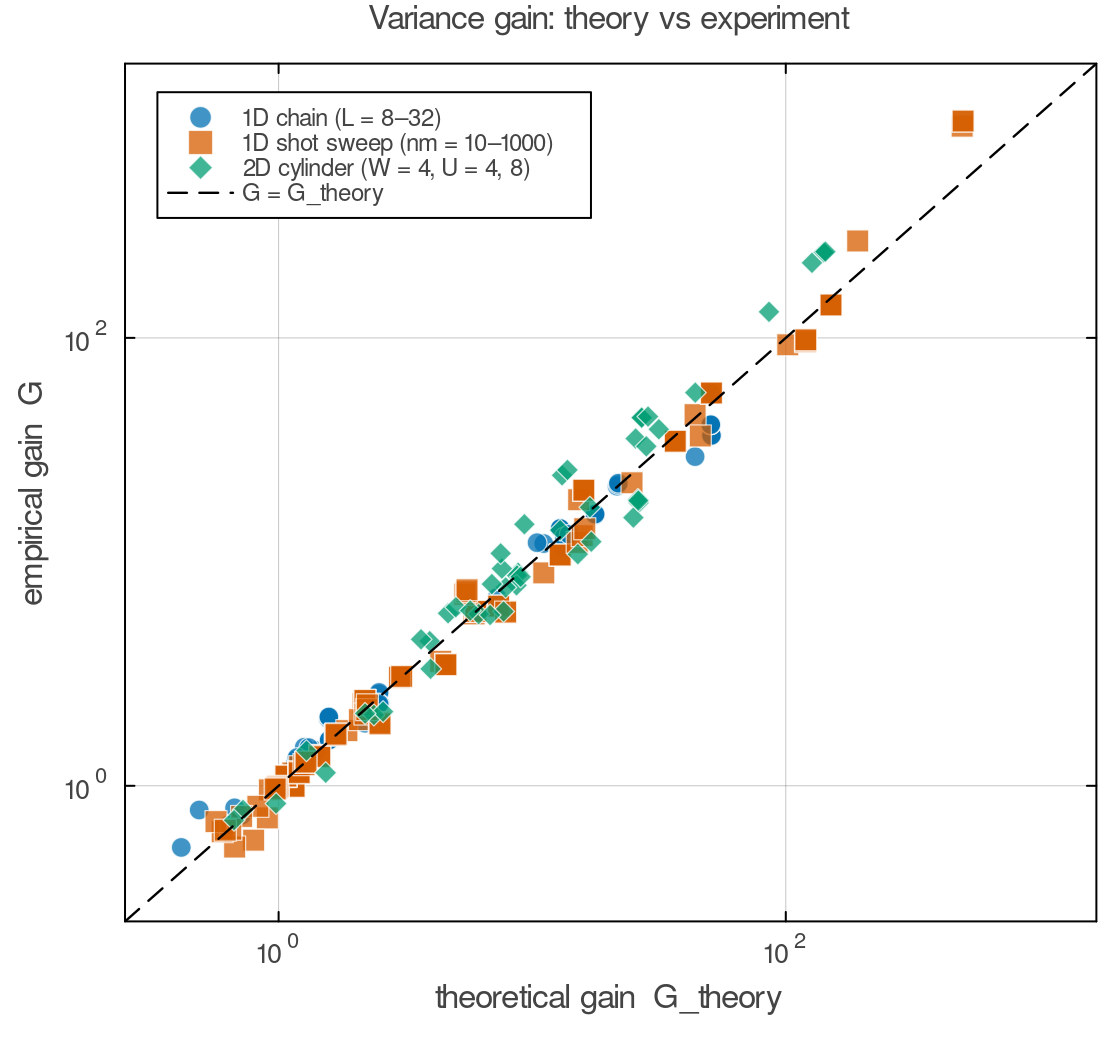
\includegraphics[width=0.62\linewidth]{crm_fig1_gainlaw.png}
\caption{利得法則のマスタープロット。1 次元鎖($L$ 掃引)、ショット配分掃引、2 次元シリンダー($U=4,8$)の全純 Pauli 列(計 218 点)について、経験利得 $G$ と理論値 \eqref{eq:gainlaw} が対角線上に乗る(約 5 桁)。}
\label{fig:gainlaw}
\end{figure}

\subsection{局所性: 忠実度崩壊下でも利得は生き残る}
\label{sec:locality}
1 次元鎖 $L=8,16,32$($U=4$、prior は $\rho$ の $\chi$ 切断)で、prior のグローバル忠実度は $F\sim f^L$ で指数的に崩壊するのに、局所観測量の利得は $L$ に対して平坦であった(表\ref{tab:locality}、図\ref{fig:locality}(a))。$L=32$ では忠実度 $F=0.0069$(ほぼ直交)の prior でも局所観測量の測定コストを 1 桁以上削減できる。一方、忠実度推定そのものは $L=8$(16 量子ビット)で既に標準シャドウの誤差 $\pm0.43$(5000 ショット)と破綻気味であり、大きい系では局所観測量への適用が本筋であることを裏づける。ショット配分依存(図\ref{fig:locality}(b))は飽和則 \eqref{eq:saturation} と一致する。

\begin{table}[t]
\centering\small
\caption{局所性の実証($U=4$、1 次元鎖)。$G$ は利得。}
\label{tab:locality}
\begin{tabular}{@{}cccccc@{}}
\toprule
$L$ & $F(\chi{=}2)$ & $G$: $ZZ\,r{=}1$ ($\chi{=}2$) & $G$: $S^zS^z\,r{=}1$ ($\chi{=}2$) & $G$: onsite $ZZ$ ($\chi{=}16$) \\
\midrule
8  & 0.35   & 12.1 & 6.1  & 36.7 \\
16 & 0.097  & 11.6 & 13.9 & 41.0 \\
32 & \textbf{0.0069} & \textbf{13.3} & \textbf{12.2} & \textbf{56.7} \\
\bottomrule
\end{tabular}
\end{table}

\begin{figure}[t]
\centering
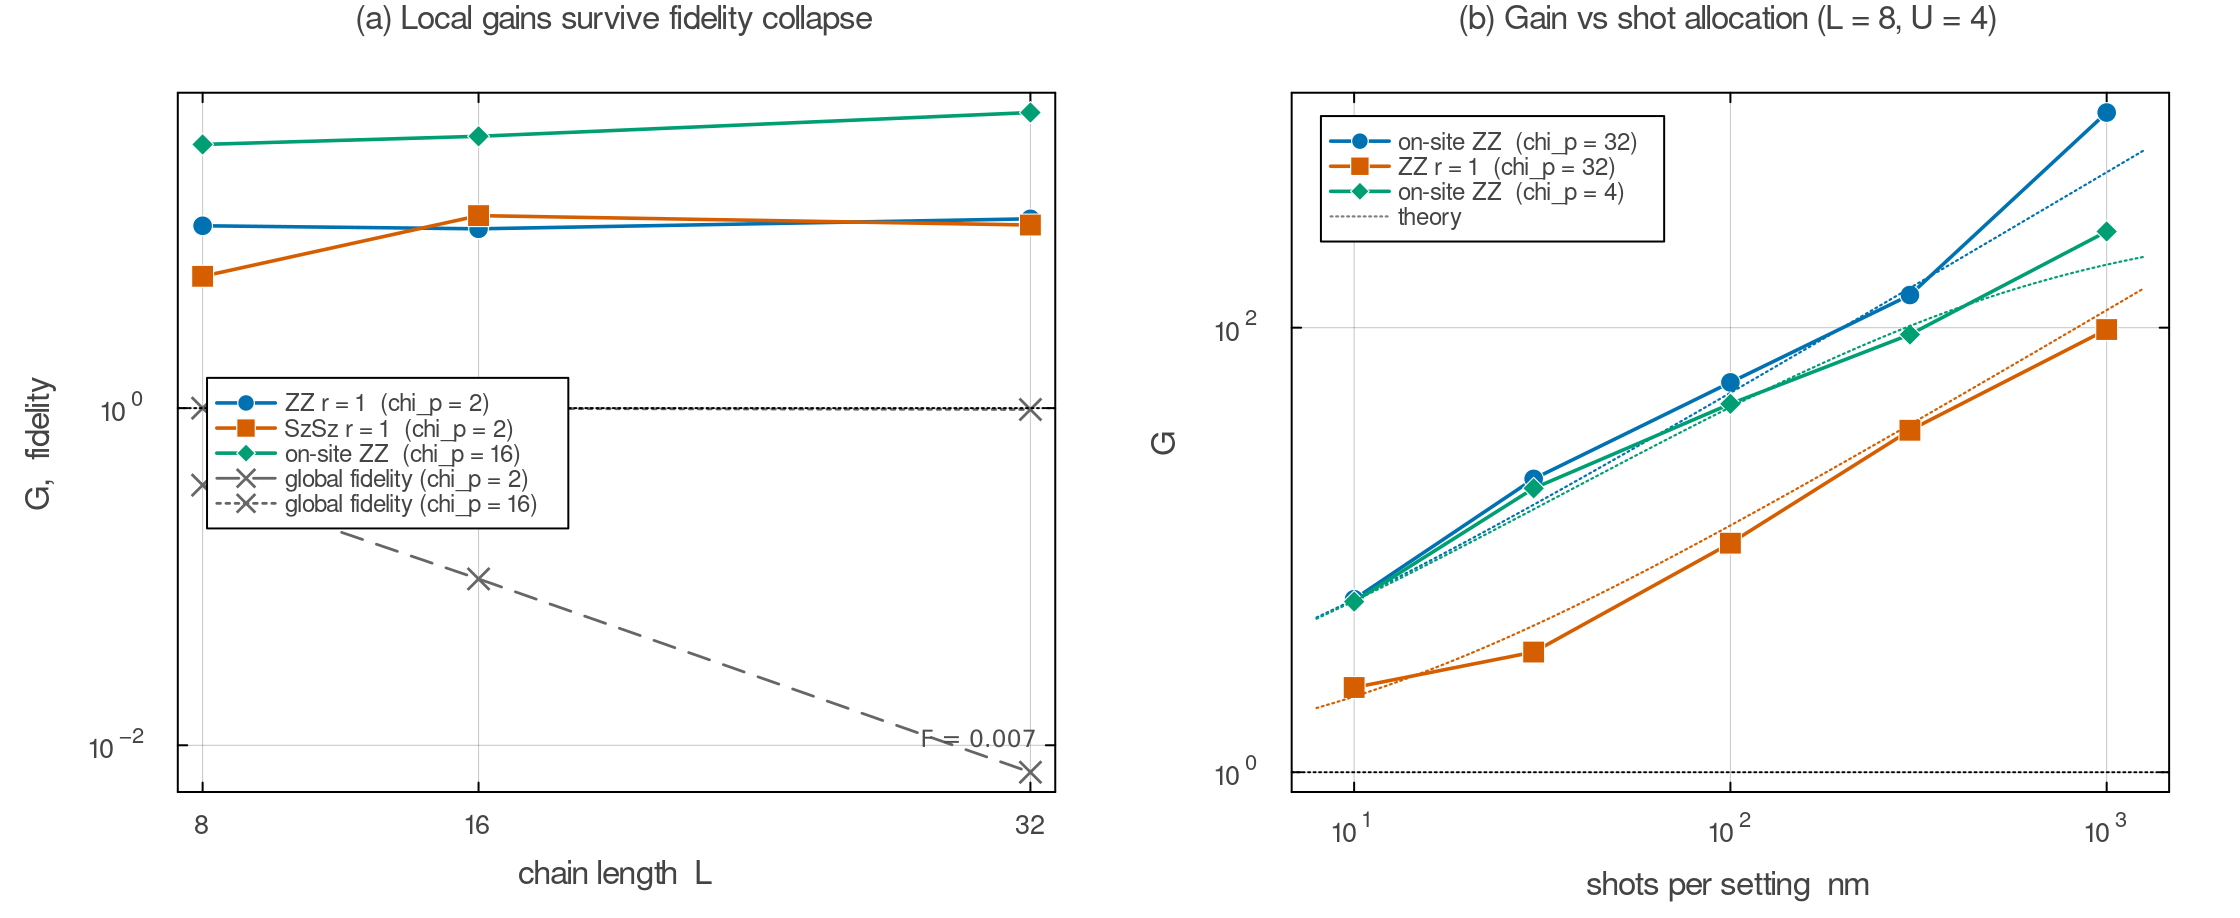
\includegraphics[width=0.95\linewidth]{crm_fig2_locality.png}
\caption{(a) $\chi{=}2$ prior のグローバル忠実度が $L$ とともに $0.007$ まで崩壊する中、局所観測量の利得は平坦。(b) ショット配分依存と飽和則の理論曲線($L=8$, $U=4$)。}
\label{fig:locality}
\end{figure}

\paragraph{解釈.}グローバル忠実度は全サイトの誤差の積なので必ず指数的に死ぬが、局所観測量の $\Delta$ はその観測量周辺の縮約密度行列の誤差だけで決まり $L$ に依存しない。相関距離を伸ばすと利得が $1$ に向かうのは、prior が悪化するのではなく $\ev{P}$ 自体が小さくなり打ち消すべき揺らぎが消えるためである。$\chi_p$ に対する利得の飽和はショットノイズ床の現れで、prior をこれ以上良くしても無駄になる点が測定予算 $n_m$ で決まることを意味する。

\subsection{相関強度・ドーピング依存}
$L=16$ の $U$・ドーピング掃引($\chi{=}8$ prior)では、利得の観測量マップが物理をそのまま反映した(表\ref{tab:phasedep})。弱結合(金属的)では運動エネルギーが大きな $\ev{P}$ を持ち、強結合(Mott)では密度・スピンが主役になる。$U=1$ やドープ系では基底状態のエンタングルメントが大きく、同じ $\chi$ の切断 prior の忠実度が下がる。

\begin{table}[t]
\centering\small
\caption{相関強度・ドーピング依存($L=16$、$\chi{=}8$ prior での $G$)。}
\label{tab:phasedep}
\begin{tabular}{@{}lccccc@{}}
\toprule
領域 & prior 忠実度 & onsite $ZZ$ & 二重占有 & ホッピング \\
\midrule
$U=1$(弱結合) & 0.81 & 2.8 & 2.1 & \textbf{45.8} \\
$U=4$ & 0.95 & 44.2 & 22.5 & 23.8 \\
$U=8$(Mott) & 0.98 & \textbf{466.7} & 160.5 & 9.5 \\
$U=4$ doped ($n{=}7/8$) & 0.80 & 15.6 & 18.7 & 43.4 \\
\bottomrule
\end{tabular}
\end{table}

\subsection{2 次元: 安価な平均場 prior は MPS prior に代われるか}
\label{sec:2d}
$4\times8$ シリンダー(64 量子ビット、half-filling、$\rho=$ DMRG $\chi=192$)で、$O(N^3)$ の UHF/UHF-sym prior(第\ref{sec:wick}節)と $\chi$ 切断 MPS prior を\emph{同一の測定データ}で比較した。前提として 2 次元では MPS prior が急劣化する($U=4$: $\chi{=}8$ で $F=0.055$、1 次元 $L=16$ の同 $\chi$ は $0.95$)。結果(表\ref{tab:2d}、図\ref{fig:2d})は次の通り。
\begin{itemize}
  \item オンサイト量と運動項では\textbf{タダの UHF が $\chi=32$--$64$ の MPS prior と同等}($U=8$ の onsite $ZZ$ で $G(\text{UHF})=241$ vs $\chi{=}64$ の $243$)。
  \item サイト間スピン相関では素の共線 UHF は失敗($G\le3$、時に $<1$):凍結 Néel 秩序が $|\ev{S^zS^z}|$ を過大評価する($\Delta\approx0.2$--$0.4$)。
  \item スピン回転平均した混合状態 prior(UHF-sym)がこの弱点を全て修復する。回転不変な観測量は厳密に不変のまま(理論予言と一致)。
  \item 例外は二重占有の退行($6.6\to3.4$)。演算子は SU(2) 不変で合計 $\Delta$ は両 prior で同一なのに $G$ が変わるのは、$\chi=192$ 参照自体が Néel 対称性を破っており項ごとの $\ev{Z_q}$ は共線 UHF の方が合うため(第\ref{sec:variance}節の「項ごと $\Delta$」)。
\end{itemize}

\begin{table}[t]
\centering\small
\caption{$W=4$ シリンダー($U=4$)での prior 比較($G$)。太字は同一観測量での最良に近い安価 prior。}
\label{tab:2d}
\begin{tabular}{@{}lcccc@{}}
\toprule
観測量 & $G$(UHF 共線) & $G$(UHF-sym) & $G$($\chi{=}16$) & $G$($\chi{=}64$) \\
\midrule
onsite $ZZ$ & \textbf{44.0} & 44.0 & 13.9 & 44.5 \\
二重占有 & 6.6 & 3.4 & 10.5 & 34.2 \\
ホッピング & \textbf{11.8} & 11.8 & 15.4 & 15.4 \\
$ZZ$ $x$隣 & 0.83 & \textbf{8.69} & 5.8 & 8.6 \\
$S^zS^z$ $x$ & 0.81 & \textbf{6.11} & 3.9 & 6.9 \\
\bottomrule
\end{tabular}
\end{table}

\begin{figure}[t]
\centering
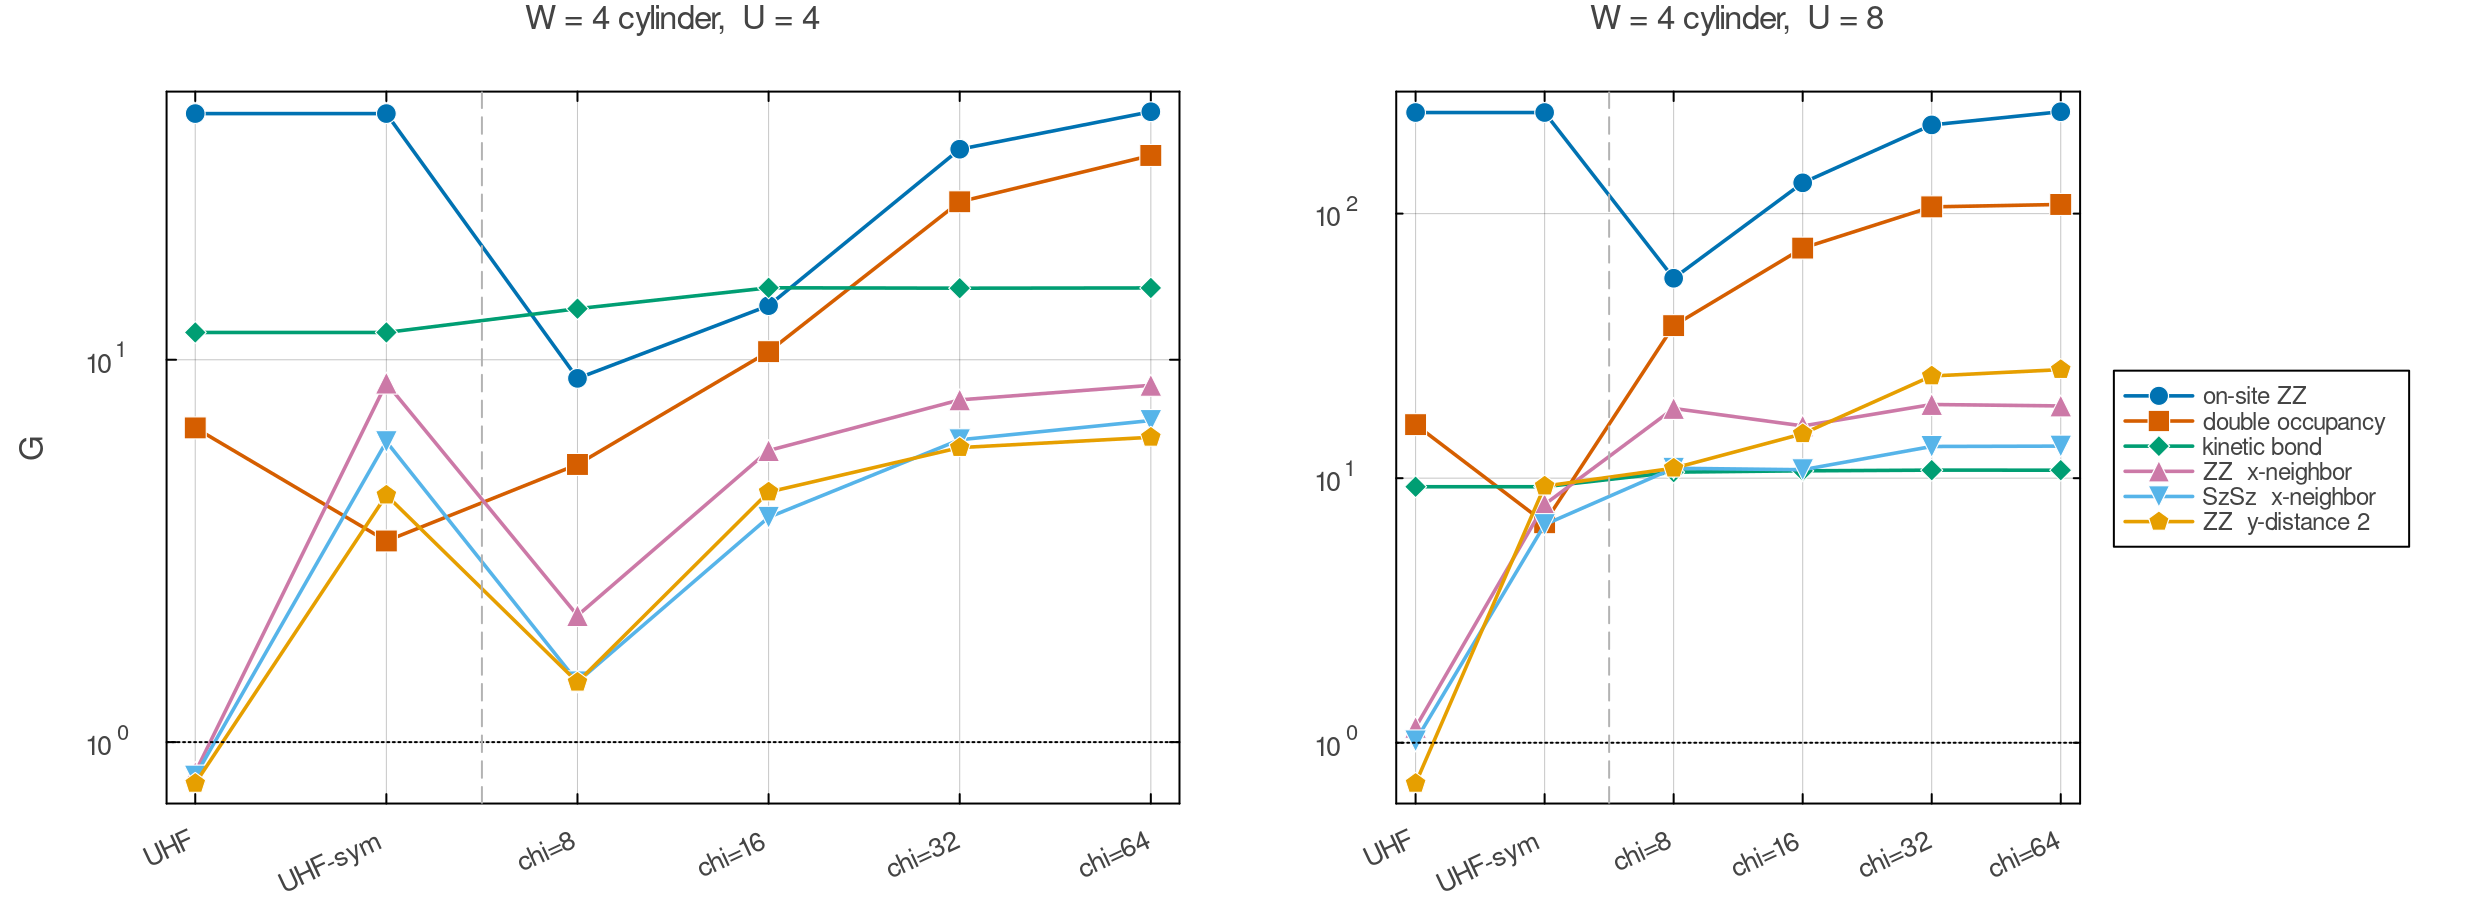
\includegraphics[width=0.95\linewidth]{crm_fig3_priors2d.png}
\caption{$W=4$ シリンダーでの prior 比較($U=4,8$)。横軸左から UHF / UHF-sym /(縦破線)/ 切断 MPS $\chi=8$--$64$。対称性回復でサイト間スピン相関(桃・水色・橙)が MPS 系に並ぶ。}
\label{fig:2d}
\end{figure}

\paragraph{W=6 へのスケールアップ(96 量子ビット、クラスター計算).}$6\times8$ シリンダー($\rho=$ DMRG $\chi=512$、研究室クラスターの PBS ジョブ)では、MPS prior の劣化がさらに加速する($U=4$: $\chi{=}8$ で $F=0.018$、$\chi{=}32$ で $0.22$)一方、UHF は持ちこたえる($U=8$ の onsite $ZZ$ で $G(\text{UHF})=157 > G(\chi{=}32)=96$)。幅 $W$ を増やすと同じ忠実度に必要な $\chi$ が指数的に増えるため、\textbf{タダの prior の相対優位はまさに MPS が苦しくなる領域で拡大する}(図\ref{fig:w6})。なお $W=6$ では共線 UHF がサイト間スピン相関でも機能し UHF-sym を上回る逆転が起きる。これは 96 量子ビットに対し $\chi=512$ が未収束で、参照自体が $W=4$ より強く Néel 対称性を破っているためで、「prior の対称性は状態の破れの程度に合わせる」という指針の再確認である。

\begin{figure}[t]
\centering
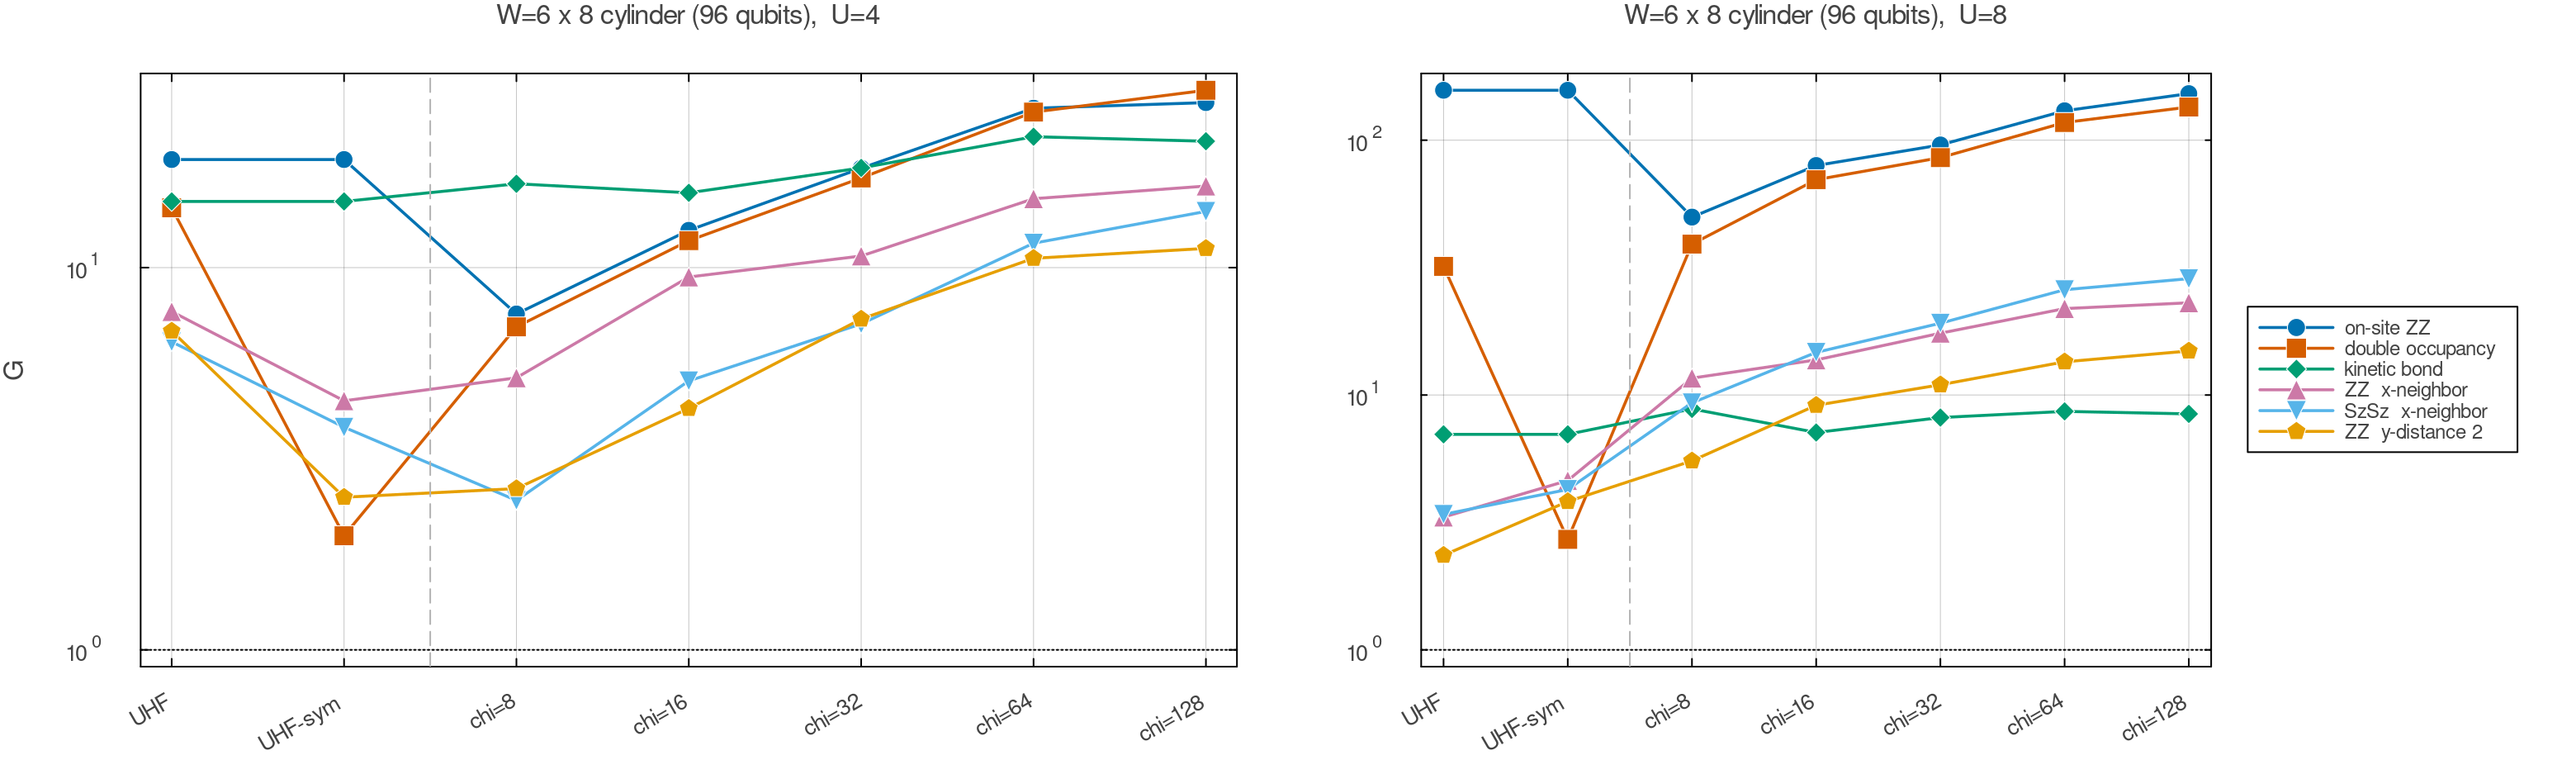
\includegraphics[width=0.95\linewidth]{crm_2d_w6.png}
\caption{$W=6$ シリンダー(96 量子ビット、クラスター計算)。安価 prior(UHF/UHF-sym)と切断 MPS の利得。$W=4$ に比べ MPS prior の立ち上がりが遅く、平均場の相対優位が拡大する。}
\label{fig:w6}
\end{figure}

\subsection{損をしない CRM: 最適係数と多 prior 回帰}
\label{sec:optbeta}
第\ref{sec:cv-method}節の最適係数化を $W=4$ シリンダー(第\ref{sec:2d}節と同一データ)で検証した(図\ref{fig:optbeta})。$\beta=1$ で損をしていた全ケースが修復され($U=8$ の UHF で $ZZ$ $y$距離2: $0.70\to13.95$、$ZZ$ $x$隣: $1.14\to18.59$)、達成利得は理論 $1/(1-\mathrm{corr}^2)$ と対角線上で一致、プラグインバイアスは検出限界以下であった。理論的副産物として、単一 Pauli 列では $Y_p=\mathbf{1}[\text{一致}]\cdot3^{|A|}\ev{P}_{\sigma_p}$ が prior ごとにスカラー倍しか違わず $\beta$ に吸収されるため、最適 $\beta$ 利得は\emph{prior 非依存}になる — すなわち「一致インジケータを制御変量とする prior フリーの自己校正推定器」が定義できる。一方 prior が優秀なら $\beta=1$ が勝つ(onsite $ZZ$: $241$ vs $141$)。多 prior 回帰では、無料の prior 2 つ $\{$UHF, UHF-sym$\}$ の回帰が二重占有で $G=98$($U=8$)に達し、$\chi=32$ MPS($101$)と同等となった — \textbf{MPS なしで MPS 級}。

\begin{figure}[t]
\centering
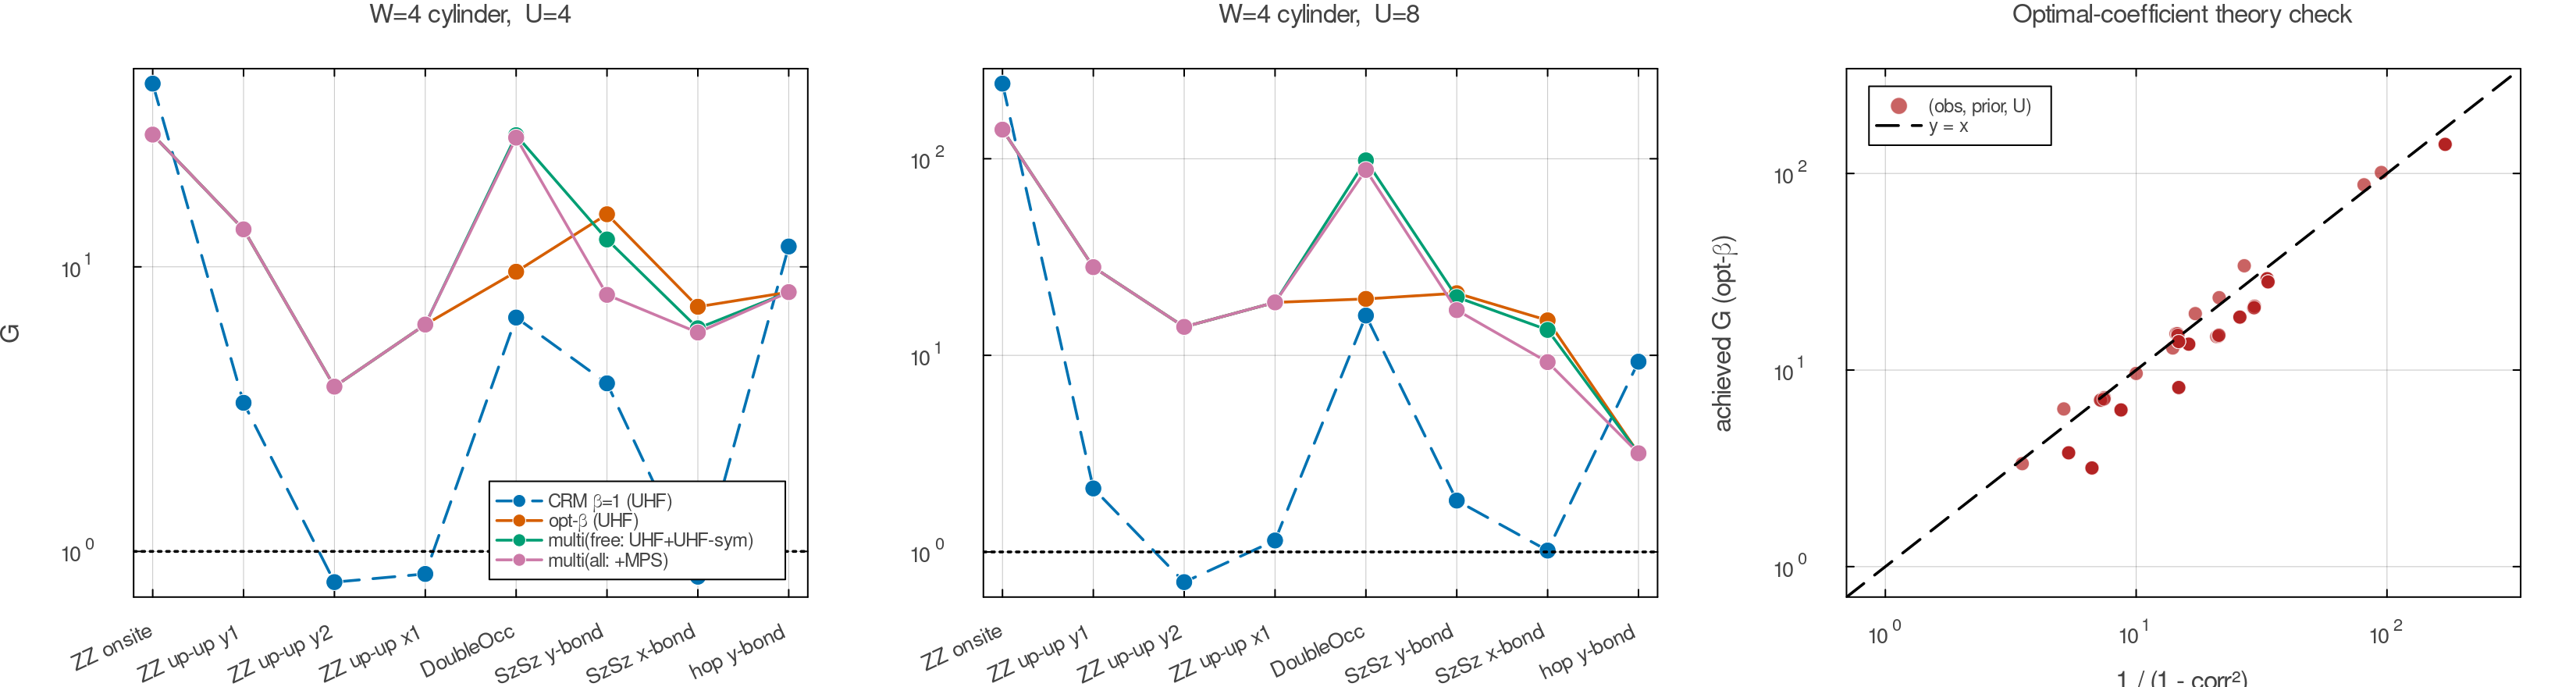
\includegraphics[width=0.95\linewidth]{crm_optbeta.png}
\caption{最適係数 CRM と多 prior 回帰($W=4$、$U=4,8$)。$\beta=1$ で $G<1$ だった観測量が最適 $\beta$ で全て $G\ge1$ に修復(右パネルで達成 $G$ が理論 $1/(1-\mathrm{corr}^2)$ に一致)。}
\label{fig:optbeta}
\end{figure}

\subsection{matchgate シャドウ: JW 弦問題と CRM の適用範囲}
\label{sec:matchgate}
$4\times2$ シリンダー(16 量子ビット、$2^{16}$ 次元密ベクトルで厳密シミュレーション)で Pauli シャドウ($\pm$CRM)と matchgate シャドウ($\pm$CRM)を同一予算で比較した(表\ref{tab:matchgate}、図\ref{fig:matchgate})。$x$ 方向ボンドは Pauli では $|A|=9$ で基底一致確率 $3^{-9}\approx1/2\text{万}$ のため 5000 設定で\emph{一度もサンプルされない}が、matchgate では 2 次 Majorana として $y$ ボンドと同精度で測れ、全エネルギー誤差は Pauli 標準の約 13 分の 1 となる。ただし(i)測定されない項の Pauli+CRM 推定は prior の値を返すため実質バイアス推定量となり(平均 $-5.35$ vs 真値 $-5.95$)、(ii)CRM は matchgate にはほとんど効かない($G\approx0.5$--$1.6$;$n_m$ を 3000 まで増やしてもエネルギーで最大 $\sim1.9$ 倍)。

\begin{table}[t]
\centering\small
\caption{Pauli シャドウ vs matchgate シャドウ($4\times2$, $U=4$、推定の標準誤差)。}
\label{tab:matchgate}
\begin{tabular}{@{}lcccc@{}}
\toprule
観測量 & Pauli 標準 & Pauli+CRM & MG 標準 & MG+CRM \\
\midrule
hop $y$ボンド & 0.211 & 0.052 & 0.098 & 0.096 \\
hop $x$ボンド ($|A|{=}9$) & \emph{測定不能} & prior 値のみ & \textbf{0.095} & 0.076 \\
全エネルギー & 11.5 & 0.88$^\dagger$ & \textbf{0.87} & 1.01 \\
\bottomrule
\end{tabular}\\[2pt]
\footnotesize $^\dagger$ 一度も測定されない $x$ ボンド項により実質バイアスを含む。
\end{table}

\begin{figure}[t]
\centering
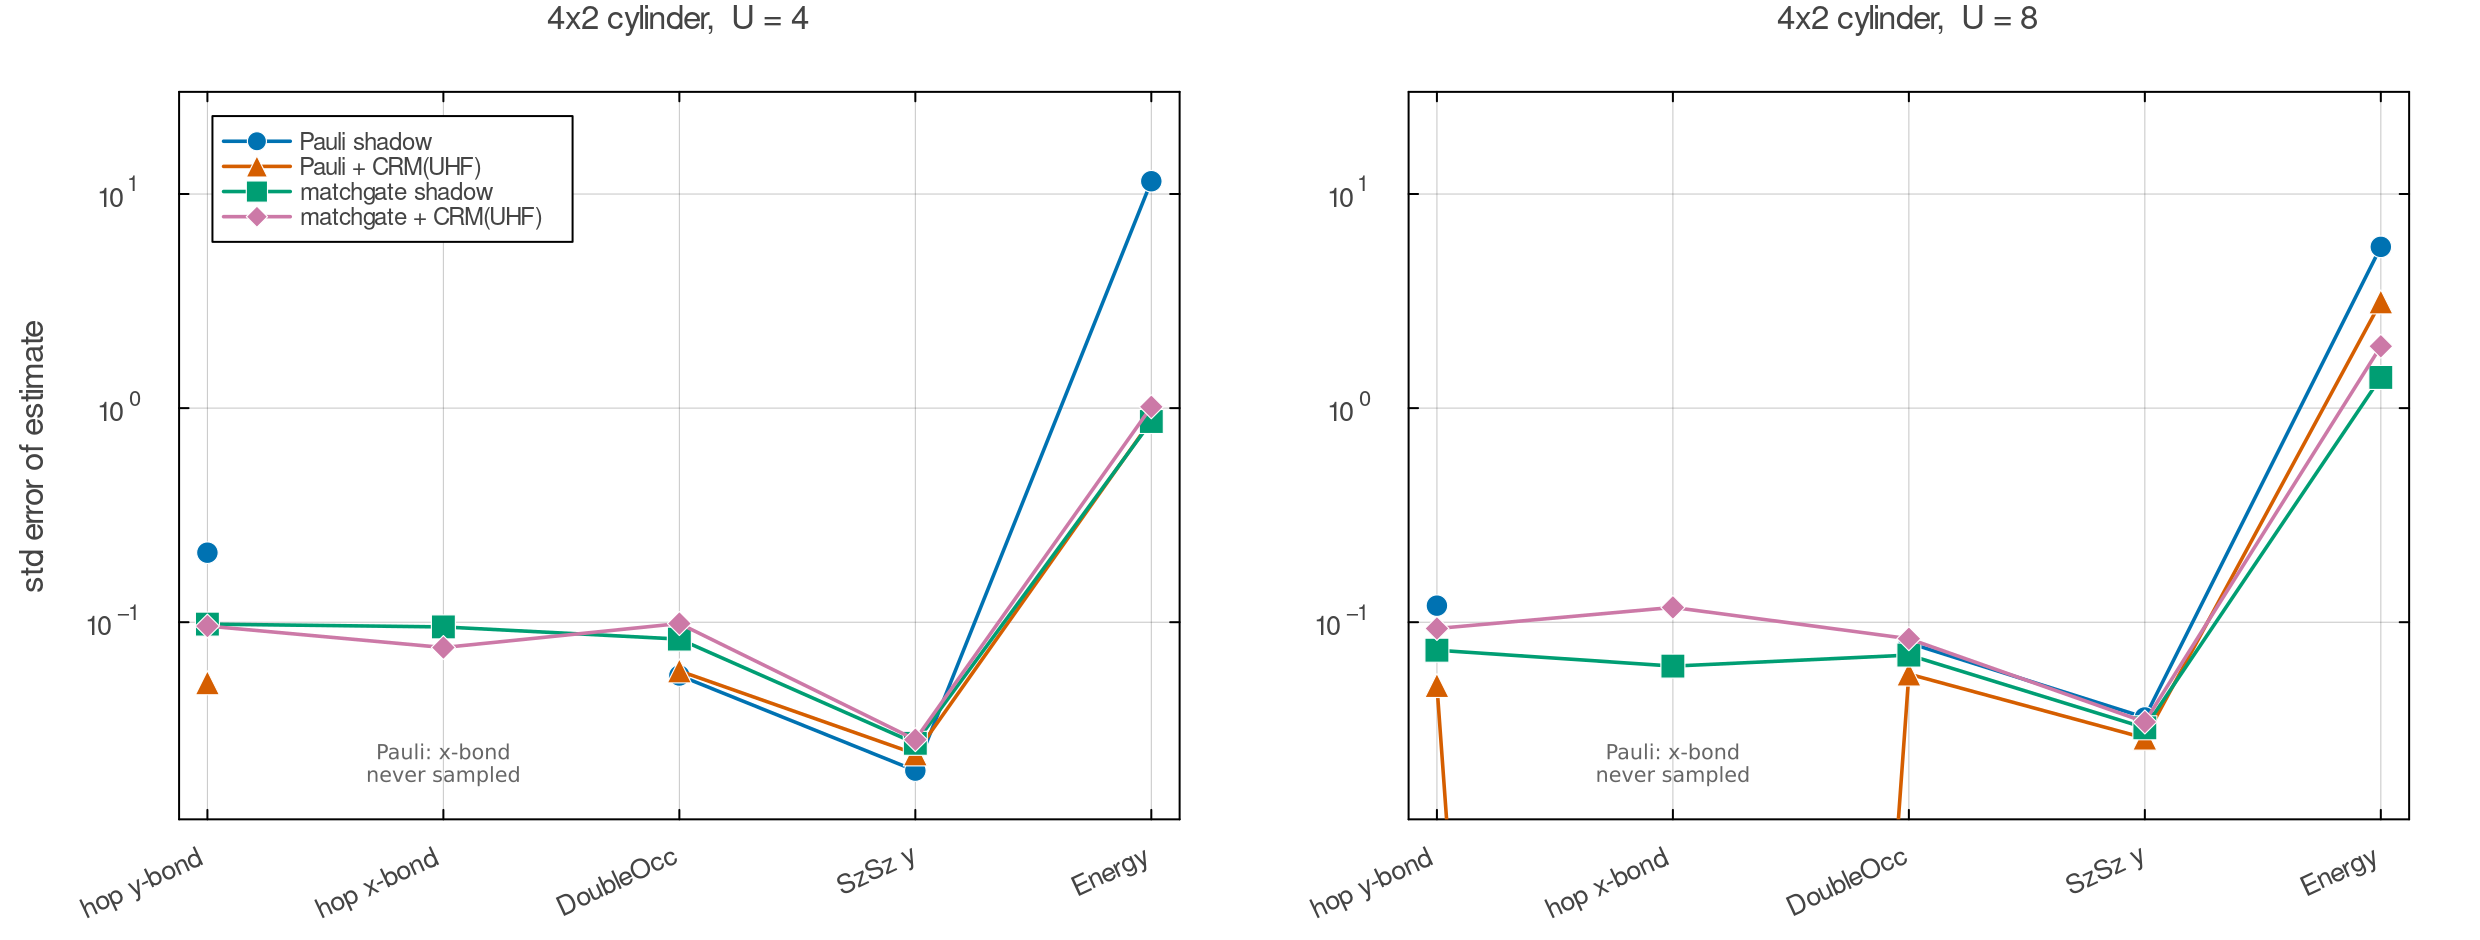
\includegraphics[width=0.95\linewidth]{crm_matchgate.png}
\caption{Pauli シャドウ / Pauli+CRM / matchgate シャドウ / matchgate+CRM の推定標準誤差($4\times2$、$U=4,8$)。Pauli の $x$ ボンドはサンプルされず表示されない。matchgate は全観測量・全エネルギーを一様に測る。}
\label{fig:matchgate}
\end{figure}

\paragraph{解釈.}Pauli シャドウの利得の源泉は「基底一致/不一致」がつくる巨大な設定間揺らぎだが、Haar 的な Gauss 回転は自己平均的でその揺らぎ自体が小さい。すなわち \textbf{CRM の価値は測定アンサンブルに依存する}。JW 弦問題は matchgate で、ランダム Pauli データの分散は CRM で、と両者は同じ問題の\emph{異なるボトルネック}に対する道具である。

\subsection{正直なベースライン: 貪欲 derandomization との比較}
\label{sec:derand}
「単一観測量なら該当基底の直接測定が最強では」という批判に答えるため、同一総ショット数(50 設定 $\times$ 100 ショット)で多数の観測量を同時推定する誤差を比較した($L=16$、$\chi{=}32$ prior)。結果(表\ref{tab:derand})、既知の固定リストには貪欲 derandomization(命中回数に指数減衰重みを付けたカバレッジ最大化)が最強である一方、CRM はシャドウの不利をほぼ帳消しにし(構造化セットで中央値 4.8 倍改善)、\emph{測定後に任意の観測量を選べる}柔軟性を保つ。非構造セットでは CRM の中央値利得は消えるが最悪誤差を半減する(誤差を支配する大 $\ev{P}$ の観測量を自動的に狙い撃つ)。決定論的設定には CRM の原理が適用不能であり、両者は相補的である。

\begin{table}[t]
\centering\small
\caption{多観測量同時推定の誤差(中央値/最悪値)。}
\label{tab:derand}
\begin{tabular}{@{}lccc@{}}
\toprule
セット & shadow 標準 & shadow+CRM & 貪欲 derand \\
\midrule
A: 構造化 23 観測量 & 0.059 / 0.351 & 0.012 / 0.054 & \textbf{0.0085 / 0.028} \\
B: ランダム 150 観測量 & 0.058 / 0.208 & 0.057 / \textbf{0.096} & \textbf{0.044 / 0.067} \\
\bottomrule
\end{tabular}
\end{table}

\subsection{ドープ系と「安価な prior の相図」の境界}
\label{sec:doped}
$1/8$ ホールドープのシリンダー($W=4\times8$ / $W=6\times8$、$\rho=$ DMRG $\chi=512$、クラスター計算)を調べた。UHF は複数初期値(Néel / ストライプ / 乱数)の競争から最低エネルギー解を採り、$W=6$・$U=8$ では教科書的な bond-centered 反位相ストライプ(ホールの川と壁を跨ぐ反強磁性の符号反転)を自発的に選ぶ。主な知見は次の通り。
\begin{itemize}
  \item \textbf{$W=4$ ドープ($U=8$)}: half-filling と逆転し、共線 UHF がサイト間スピン相関で大失敗($\Delta\approx0.44$--$0.56$)、UHF-sym が救う($ZZ$ $y$隣 $0.6\to12.0$)。ドープ状態は静的秩序が溶けてより対称的なので対称化 prior が合う。
  \item \textbf{$W=6$ ドープ($U=8$)}: 破綻が電荷テクスチャに局在する。観測窓を壁の上(x=4)からドメイン内(x=2)へ移すと UHF-sym がスピン相関を再び $\chi=16$--$32$ MPS 相当まで救う($\Delta\approx0.01$--$0.03$)。一方\emph{サイト分解密度}(ストライプ秩序パラメータ)はどの平均場 prior でも不可($G\approx0.1$):UHF のストライプは電荷変調が鋭すぎ、揺らぎで軟化した DMRG 参照と合わない。
  \item 運動ボンドは全領域・全 prior で常に容易($G\approx6$--$23$)。
\end{itemize}
以上を統合すると、安価な平均場系 prior の有効領域は「秩序が強く(ほぼ)一様な状態」— half-filling は任意幅で共線 UHF、ドープ強結合のスピンセクターはドメイン内で対称性回復 UHF が機能する。\textbf{破綻は広幅ドープ系の電荷テクスチャに局在}し、そこでは $\chi\ge32$ の MPS か平均場を超える prior(電荷分布を拘束した平均場、Gutzwiller/DMET 的)が必要である。どの領域でも最適 $\beta$ CRM(第\ref{sec:optbeta}節)が「損はしない」保険として下支えする。

\section{考察と展望}

本研究の一貫した主張は、\textbf{CRM の利得は prior のグローバルな良さではなく、測りたい観測量に対する局所的な良さ $\Delta$ で決まる}という点である(閉形式 \eqref{eq:gainlaw})。ここから、(i) 系を大きくしても局所観測量なら利得が保たれること、(ii) MPS を要さない平均場 prior が 2 次元で MPS prior に匹敵すること、(iii) 混合状態 prior という自由度が実際に有用であること、が導かれた。さらに CRM を制御変量法へ一般化することで「損をしない」保証を得、matchgate シャドウ・derandomization との\emph{相補性}を明確にした。「安価な prior の相図」は、次に作るべき prior(電荷テクスチャを捉える中間コスト prior)の設計指針を与える。

主要な残課題は、(a) prior を測定計画自体の設計に用いる prior-informed derandomization、(b) 最終図へのブートストラップ信頼区間、(c) 時間依存平均場(TDHF)/有限温度 Gauss 状態を prior とする動力学・熱平衡への拡張、(d) matchgate アンサンブルの分散理論(CRM がいつ効くかの定量化)、(e) 電荷分布を拘束した平均場 prior、である。実装は全て自己完結の Julia スクリプトとしてリポジトリに整備されており、クラスター(PBS)実行にも対応する。

\section*{再現性}
全数値実験は \texttt{examples/tatsuyama/} 下の自己完結 Julia スクリプトで再現できる。局所実行は
\begin{center}
\texttt{JULIA\_LOAD\_PATH="@:@v\#.\#:@stdlib" julia --project=Hubbard\_MPS\_Env\_v2 <script>.jl}
\end{center}
クラスター実行は \texttt{qsub -v UVAL=8.0 <script>.pbs}。詳細な実験記録は \texttt{README.md}、論文構成の整理は \texttt{CRM\_RESEARCH\_NOTES.md} を参照。

\begin{thebibliography}{9}
\bibitem{crm} B.~Vermersch \textit{et al.}, ``Enhanced estimation of quantum observables with common randomized measurements,'' PRX Quantum \textbf{5}, 010352 (2024).
\bibitem{shadow} H.-Y.~Huang, R.~Kueng, J.~Preskill, ``Predicting many properties of a quantum system from very few measurements,'' Nat.\ Phys.\ \textbf{16}, 1050 (2020).
\bibitem{derand} H.-Y.~Huang, R.~Kueng, J.~Preskill, ``Efficient estimation of Pauli observables by derandomization,'' Phys.\ Rev.\ Lett.\ \textbf{127}, 030503 (2021).
\bibitem{matchgate1} Z.~Zhao, N.~C.~Rubin, A.~Miyake, ``Fermionic partial tomography via classical shadows,'' Phys.\ Rev.\ Lett.\ \textbf{127}, 110504 (2021).
\bibitem{matchgate2} K.~Wan, W.~J.~Huggins, J.~Lee, R.~Babbush, ``Matchgate shadows for fermionic quantum simulation,'' Commun.\ Math.\ Phys.\ (2023).
\bibitem{fw} M.~T.~Fishman, S.~R.~White, ``Compression of correlation matrices and an efficient method for forming matrix product states of fermionic Gaussian states,'' Phys.\ Rev.\ B \textbf{92}, 075132 (2015).
\end{thebibliography}

\end{document}
